\section{Online Estimation Tool for ML jobs}
\label{sec:res_estimation}

%We present the online profiling tool for ML jobs in this section.
%The tool is to pick the resource configurations for jobs on CPU and GPU.

Job performance is often unknown before it actually finishes.
The performance depends on the job itself, the runtime environment, and the allocated resources.
Fortunately, ML (machine learning) jobs are iterative and predictable.
To pick the best resource configurations for an ML job, the tool uses the shorter versions of the job to estimate the performance and resource configurations.
Unlike Ernest \cite{ernest} and CherryPick \cite{cherrypick}, we do not estimate the number of nodes for a job.
Instead, we estimate the job performance and the resource configurations of a job that fits within the a node.
It is because most of ML models can be fit in the a single node. Furthermore, if the ML job is distributed, the tool can be used for each distributed task.

\begin{figure}[h]
	\centering
	%    
\includegraphics[width=0.6\linewidth]{fig/b1i3_res_usage_legend} 
	\subfloat[] {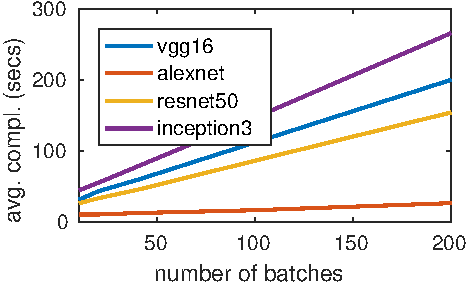
\includegraphics[width=0.45\linewidth]{figs/prof-batchnum-gpu} \label{fig:prof-batchnum-gpu}}    \hspace{0.0in}
	\subfloat[] {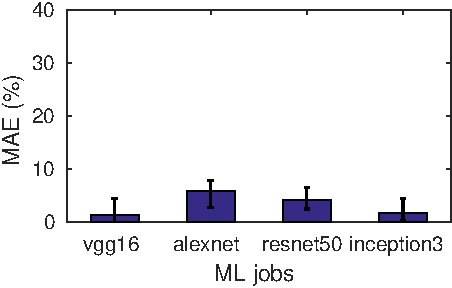
\includegraphics[width=0.45\linewidth]{figs/beta_est_gpu} \label{fig:beta_est_gpu}} 
	\caption{(a) The completion times of jobs linearly increase with respect to number of batches. (b) Running 2 short versions of a job can predict the job completion times under 7\% error.}
	\label{fig:est_compl_time}
\end{figure}



%\subsection{Online profiling tool}
\desc{How the current tool version works?}

\emph{Inputs.} The job inputs are kept in text files where each file has a list of jobs.
Each file represents for a user.
Each job has a CPU configruation and a GPU configuration.

\emph{Sampling.} If we want to predict the processing time of an ML job on CPU, we create 2 sampled version of jobs.
The two samples are $a\%$ and $b\%$ of the original job.
The ML jobs are iterative and they have a lot of batches because the trained dataset is very large compared to the physical memory.
If the number of batches is too small, the overhead on job initialization may have impact on the job performance.
In practice, the ML jobs are often very long because they need to train on a large dataset.
Each sampled version is configured with maximum possible resources because we do not know the resource configuration for the job yet.

We implement the tool using Python.
Roughly 1000 lines of Python code were written.
The tool reads the input jobs from users.
Jobs are command-line based.
Meaning, users can submit the jobs by passing parameters via command lines.
The parameters allow us to scale down the jobs and create the small samples.
In this paper, we use the number of batches that indicates how many batches that will be fed to ML models.
We can extend this one to amount of data.
After the tool measures the completion times of samples, it estimates the job performance via linear regression.
It also picks the best resource configurations for the job.
Finally, it submits the job with the best configurations and the estimated performance.

\emph{Workload Collection.} \todo{add details}

\desc{How estimate the performance of the full job?}

To demonstrate the accuracy of the method,
we run 2 short versions ($5$\% and $10$\% of the number of batches) of each job and use a linear model to estimate the completion times of the full job.
Figure \ref{fig:prof-batchnum-gpu} shows that the completion times of ML jobs linearly increase when the number of batches goes up.
This gives us the confidence to create a shorter version (a small number of batches or small datasets) to estimate the performance of the full job.
Figure \ref{fig:beta_est_gpu} shows that the simple approach works well as the errors are below 7\%.

\subsection{How to pick the CPU requests?}

%\subsection{Picking CPU configuration}
%\label{sec:pick_cpu_conf}

%Although a user is allowed to setup his own job, we offer him the way pick the CPU configuration for the job.
%The CPU configuration includes: the number of CPU cores and the amount of memory that the job needs.


\desc{How to pick CPU request?}

%We run a few Tensorflow benchmark jobs \cite{tensorflow-benchmark} on CPU Xeon E5 20 cores.
%To see the impact of CPU cores on the job completion time,
%we vary the the allocation of number of CPU cores for each job from 1 to 
%19 cores.
%Figure \ref{fig:prof_cpu_speedup} shows the number of CPU cores plays an important role in ML jobs.
%The speed-up is computed based on how much faster a job running on multiple CPU cores v.s. running the job on a single CPU core is.
%The performance significantly increases as the jobs have more CPU cores.
%Machine learning frameworks like Tensorflow or Caffe allow us to enable mutilple threads so that the use multiple CPU cores to improve the performance.
%Hence, we should pick the largest number of CPU cores possible to have the optimal job performance as well as save other resources.
%
%\begin{figure}[h]
%	\centering
%	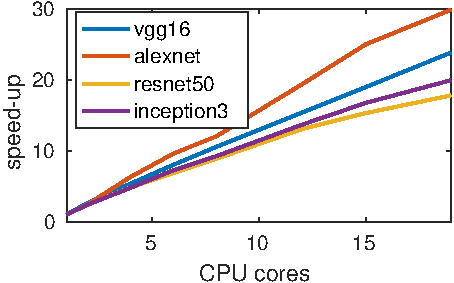
\includegraphics[width=0.7\linewidth]{figs/prof_cpu_speedup}
%	\caption{Using more CPU cores can improve the performance of ML jobs significantly .}
%	\label{fig:prof_cpu_speedup}
%\end{figure}

\begin{figure}[h]
	\centering
	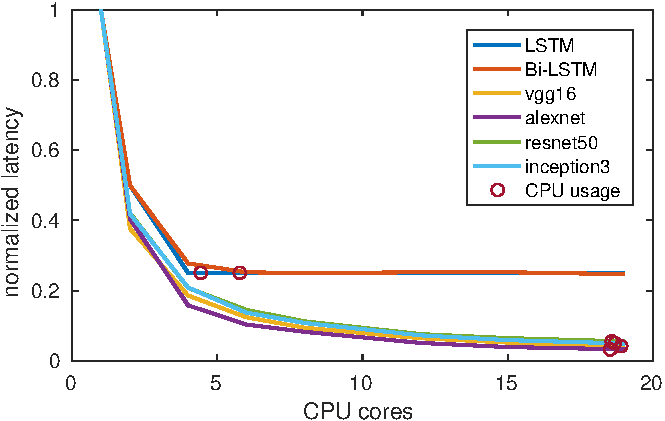
\includegraphics[width=0.7\linewidth]{figs/pick_cpu_cores}
	\caption{Using the maximum CPU usage of the sampled versions can maxi}
	\label{fig:pick_cpu_cores}
\end{figure}

Figure \ref{fig:pick_cpu_cores} shows that we can use the maximum CPU usage as the CPU requests for an ML job.
As the sampled version is running, we pick the maximum CPU usage (in percentage, 300\% means 3 cores).
Than, we compares the performance of picked CPU requests and the performance of the jobs when varying the CPU demand.

While CPU configurations do not need GPUs, GPU configurations still need CPU cores to coordinate the computation and I/O transfers between GPU and other resources like memory.
Figure \ref{fig:cpu_on_gpu} shows the impact of the number of CPU cores on the performance of Alexnet job. 
We still need more than a single CPU core to help GPU jobs achieves the best performance.
Many CPU cores are not necessary as the job completion time remains constant.

\begin{figure}[h]
	\centering
	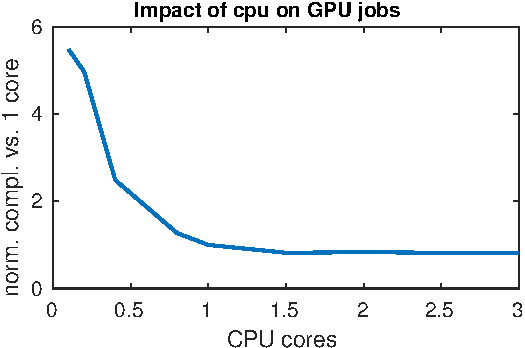
\includegraphics[width=0.7\linewidth]{figs/cpu_on_gpu}
	\caption{Applications running on GPUs also require CPUs as some computation needs to be done on CPUs.}
	\label{fig:cpu_on_gpu}
\end{figure}

\subsection{How to pick memory request?}

\desc{How memory impacts on job completion times?}

Figure \ref{fig:prof-mem-64-cpu} shows the completion times of each job when we vary the memory allocation for each job.
The out of memory errors incur when the allocated memory is too small so we do not have the completion times for these cases.
When memory are sufficient, the completion times of jobs actually do not change much if we allocate more memory to the jobs.

\begin{figure}[h]
	\centering
	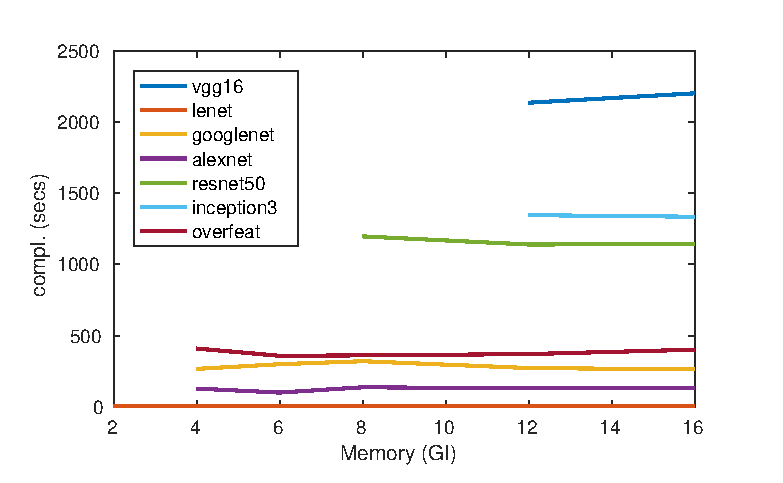
\includegraphics[width=0.7\linewidth]{figs/prof-mem-64-cpu}
	\caption{Allocating more memory does not improve the performance of the ML jobs.}
	\label{fig:prof-mem-64-cpu}
\end{figure}

\desc{How to pick memory for CPU configuration?}

\begin{figure}[!h]
	\centering
%	\vspace{-0.2in}
	\subfloat[] {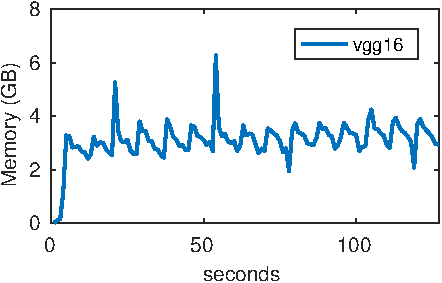
\includegraphics[width=0.45\linewidth]{figs/mem_usage_logcpu} \label{fig:mem_usage_logcpu}}    \hspace{0.1in}
	\subfloat[] {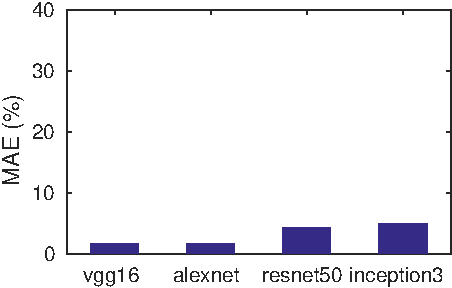
\includegraphics[width=0.45\linewidth]{figs/mem_usage_errcpu} \label{fig:mem_usage_errcpu}} 
	%	\vspace{-0.15in}
	\caption{(a) The memory usage of an ML job has a similar pattern overtime (b) Averaging the memory usage of the short versions can estimate the memory usage average of the job at high accuracy.}
	\label{fig:mem_usage}
\end{figure}

Figure \ref{fig:mem_usage_logcpu} shows memory usage of VGG16. As ML jobs are iterative, the memory usage maintains the similar pattern over time. 
So, we can use the short versions of ML jobs to estimate the average memory usage.
Figure \ref{fig:mem_usage_errcpu} shows that we can predict the memory usage well (below 5.5\% error) using the short versions (25x shorter).

\desc{How to pick memory for GPU configurations?}

The GPU configuration often needs less main memory than the CPU configuration.
GPU are designed with their own memory to minimize the transfer overhead between GPUs and the host machine.
So, most of the computations are carried on the GPU memory while the main memory is used to coordinate the computation tasks on GPU.

\subsection{How to pick GPU?}

\desc{Justify why we do not have results on GPUs.}

A single GPU is often powerful enough to carry on a single ML job and multiple GPUs are not efficient as the communication can be the bottleneck \cite{tensorflow-performance}.
If picking the number of GPUs for a job is necessary, similar approaches like Ernest \cite{ernest} or CherryPick \cite{cherrypick} can be used.

\subsection{Speed-up rate estimation}

The tool estimates the speed-up rate of the job on GPU to CPU.
The speedup rates are estimated using the ratio of the completion times of two short versions.
The estimation errors are shown in Figure \ref{fig:beta_est}.
The mean absolute errors are at most 11.44\% \todo{Update the new results.}. 

\begin{figure}[h]
	\centering
	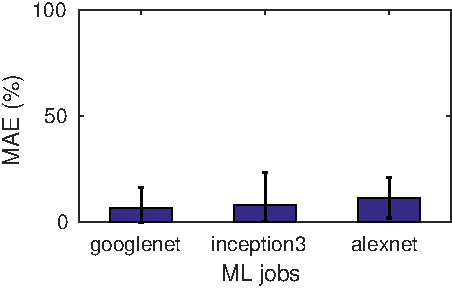
\includegraphics[width=0.5\linewidth]{figs/beta_est}
	\caption{The estimation errors of speedup rates of CPU completion times to GPU completion times.}
	\label{fig:beta_est}
\end{figure}

\todo{Additional challenge: Nodes are heterogeneous.}

\todo{Additional challenge: if the speed-up rate is high, the sampled job on CPU can last very long. In this case, it is not useful because we need to wait for the sampled jobs finished.}


\emph{Key insights:}  ML jobs are iterative that allow us to sample the jobs and estimate the speed-up rates.
%The ML jobs can be configured with multiple threads so they prefer to have more CPU cores on a node.
Memory usage of ML jobs do not change much overtime, so we can pick the resource usage for based on the sampled jobs.
GPU configurations do not requires large main memory as the computation is mainly carried on GPUs.



